\documentclass{article}

\title{babette: BEAUti 2, BEAST2 and Tracer for R}
\author{Rich\`el J.C. Bilderbeek, Rampal S. Etienne}

\usepackage{listings}
\usepackage{hyperref}
\usepackage{todonotes}
\usepackage{verbatim}
\usepackage{tikz}
\usepackage{tkz-graph}
\usepackage{pgf}
\usepackage{bm}
\usetikzlibrary{arrows,automata}

% Style of listings
% From http://r.789695.n4.nabble.com/How-to-nicely-display-R-code-with-the-LaTeX-package-listings-tp4648110.html
\usepackage{fancyvrb} 
\definecolor{codegreen}{rgb}{0,0.6,0}
\definecolor{codegray}{rgb}{0.5,0.5,0.5}
\definecolor{codepurple}{rgb}{0.58,0,0.82}
\definecolor{backcolor}{rgb}{0.95,0.95,0.92}
\lstdefinestyle{mystyle}{
  language=R,% set programming language
  basicstyle=\ttfamily\small,% basic font style
  commentstyle=\color{gray},% comment style
  % numbers=left,% display line numbers on the left side
  numberstyle=\scriptsize,% use small line numbers
  numbersep=10pt,% space between line numbers and code
  tabsize=2,% sizes of tabs
  showstringspaces=false,% do not replace spaces in strings by a certain character
  captionpos=b,% positioning of the caption below
  breaklines=true,% automatic line breaking
  escapeinside={(*}{*)},% escaping to LaTeX
  fancyvrb=true,% verbatim code is typset by listings
  extendedchars=false,% prohibit extended chars (chars of codes 128--255)
  alsoletter={.<-},% becomes a letter
  alsoother={$},% becomes other
  otherkeywords={!=, ~, $, \&, \%/\%, \%*\%, \%\%, <-, <<-, /},% other keywords
  deletekeywords={c}% remove keywords 
}
\lstset{style=mystyle}

% Adds numbered lines
\usepackage{lineno}
\linenumbers

% Rename 'Abstract' to 'Summary 
\usepackage[english]{babel}
\addto{\captionsenglish}{\renewcommand{\abstractname}{Summary}}

% Keywords
% \usepackage{spconf}

\usetikzlibrary{calc}
\usetikzlibrary{arrows.meta}

\begin{document}

\maketitle

\begin{abstract}

  \textbf{1. }
    In the field of phylogenetics, 
     BEAST2 is one of the most widely used software tools. 
     It comes with the graphical programs BEAUti 2 to
     facilitate the creation of BEAST2 configuration files, and
     with DensiTree and Tracer, to interpret BEAST2's output files. 
     However, when many different alignments or model 
     setups are required, a workflow of GUI programs is cumbersome. \\
  \textbf{2. }
    Here, we present a free, libre and open-source package, \verb;babette;, 
    'BEAUti 2, BEAST2 and Tracer for R', for the R programming language. 
    \verb;babette; creates BEAST2 input files, runs BEAST2 and parses its results, 
    all from an R function call. \\
  \textbf{3. }
    We describe \verb;babette;'s usage, the novel functionality it provides
    compared to the tools it is alternative of, and give some examples. \\
  \textbf{4. }
    As \verb;babette; is designed to be of high quality and extendable, 
    we conclude by describing the further development of the package \\
\end{abstract}

% Ideal
%\begin{keywords}
%  computational biology, evolution, phylogenetics, BEAST2, R
%\end{keywords}

% Dirty hack
{\bf Keywords:} computational biology, evolution, phylogenetics, BEAST2, R


%%%%%%%%%%%%%%%%%%%%%%%%%%%%%%%%%%%%%%%%%%%%%%%%%%%%%%%%%%%%%%%%%%%%%%%%%%%%%%%%%%%%%%
\section{Introduction}
%%%%%%%%%%%%%%%%%%%%%%%%%%%%%%%%%%%%%%%%%%%%%%%%%%%%%%%%%%%%%%%%%%%%%%%%%%%%%%%%%%%%%%

Phylogenies are commonly used to explore evolutionary hypotheses.
Not only can phylogenies show us how species (or other
evolutionary units) relate to each other, 
but also relevant parameters like extinction and 
speciation rates can be estimated from them.

There are many phylogenetics tools available to obtain an estimate 
of the phylogenetic tree of a given set of species. 
BEAST2 \cite{bouckaert2014beast} is one of the most widely used ones. 
It creates a posterior of jointly-estimated phylogenies and model parameters, 
from a DNA, RNA or amino acid alignment (see figure \ref{fig:workflow} 
for an overview of the workflow). 
It is a console application, that needs a configuration file containing 
alignments and model parameters.

BEAST2 is bundled with BEAUti 2 \cite{drummond2012bayesian} ('BEAUti' from now on), 
a desktop application to create a BEAST2 configuration file.
BEAUti has a user-friendly graphical user interface, with helpful and 
reasonable default settings.
As such, BEAUti is an attractive alternative 
to manual and error-prone editing of BEAST2 configuration files. 

BEAUti cannot be called from a command-line script.
This implies that when the user 
wants to explore the consequences of various settings, this must be done manually.
This is the common workflow when using a few alignments and doing a superficial 
analysis of sensitivity of the reconstructed tree to model settings. 

However, for exploring many trees (for instance from simulations) and for
more thorough sensitivity analysis, one would like to loop through 
multiple (simulated) alignments, nucleotide substitution models, 
clock models and tree priors. 

BEAST2 is also associated with Tracer \cite{tracer} and 
DensiTree \cite{DensiTree}. Both are desktop applications 
to analyze the output of BEAST2, each with a user-friendly graphical user interface. 

Tracer's purpose is to analyze the parameter estimates generated
from a BEAST 2 run. It shows, among
others, the effective sample size (ESS) and time series ('the trace', 
hence the name) of each variable in the MCMC run. Both ESS and trace
are needed to assess the strength of the inference. 
DensiTree visualizes the phylogenies of a BEAST2 posterior, with
many options to improve the displayal of those many phylogenies.

However, for exploring the output of many BEAST2 runs, 
one would like a script to collect all parameter ESSes,
parameter traces and posterior phylogenies. 

Here, to provide such functionality we present \verb;babette;, 
’BEAUti 2, BEAST2 and Tracer for R’, 
which creates BEAST2 configuration files,
runs BEAST2, and analyzes its results,
all from an R function call. This
will save time, tedious mouse clicking and 
reduces the chances of errors in such repetitive actions.
The interface of \verb;babette; mimics the tools it
is inspired on. This
familiarity helps both beginner and experienced BEAST2 users 
to make the step from those tools to \verb;babette;.
\verb;babette; enables the creation of a single-script 
pipeline from sequence alignments to posterior analysis in R. 

\verb;babette; is the first R package that unifies the
full workflow of working with BEAST2. An
example to create a BEAST2 input file is 
\verb;BEASTmasteR; \cite{beastmaster}.
Also \verb;BEASTmasteR; allows 
to create BEAST2 configuration files from R. 
The difference is that \verb;babette; 
has its focus on DNA alignments and ultrametric trees, 
where \verb;BEASTmasteR; is used for 
morphological traits and tip-dating.
Examples of R packages to parse the BEAST2 output files
are \verb;rBEAST; \cite{rBEAST} and 
\verb;RBEAST; \cite{RBEAST}. 

%%%%%%%%%%%%%%%%%%%%%%%%%%%%%%%%%%%%%%%%%%%%%%%%%%%%%%%%%%%%%%%%%%%%%%%%%%%%%%%%
\begin{figure}
  \centering
  \resizebox {0.8\columnwidth} {!} {
    \begin{tikzpicture}[->,>=stealth',shorten >=1pt,auto,node distance=6cm, semithick]   
    \tikzstyle{every state}=[]
    \node[state] (A) [rectangle] {
      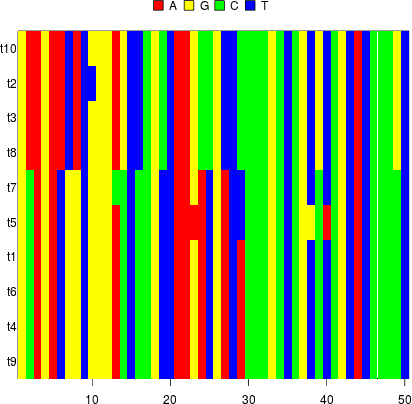
\includegraphics[width=0.2\textwidth]{alignment.png}
    };   
    \node[state] (AL) [above left=-0.25cm and -0.25cm of A, fill=white] {
      1
    };   
    \node[state] (B) [right of = A, rectangle] {
      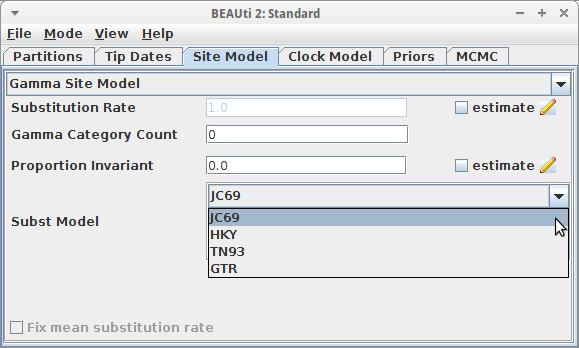
\includegraphics[height=0.15\textheight]{BeautiSiteModel.png}
    };   
    \node[state] (BL) [above left=-0.25cm and -0.25cm of B, fill=white] {
      2
    };   
    \node[state] (E) [below of=A, rectangle] {
      
\includegraphics[height=0.1\textheight]{file2.png}
    };   
    \node[state] (EL) [above left=-0.25cm and -0.25cm of E, fill=white] {
      3
    };   
    \node[state] (C) [right of = E, rectangle] {
      
\includegraphics[width=0.3\textwidth]{beast_logo.png}
    };   
    \node[state] (CL) [above left=-0.25cm and -0.25cm of C, fill=white] {
      4
    };   
    \node[state] (F) [rectangle, below of=E] {
      
\includegraphics[height=0.1\textheight]{file.png}
    };
    \node[state] (FL) [above left=-0.25cm and -0.25cm of F, fill=white] {
      5
    };   
    \node[state] (H) [rectangle, below of=F] {
      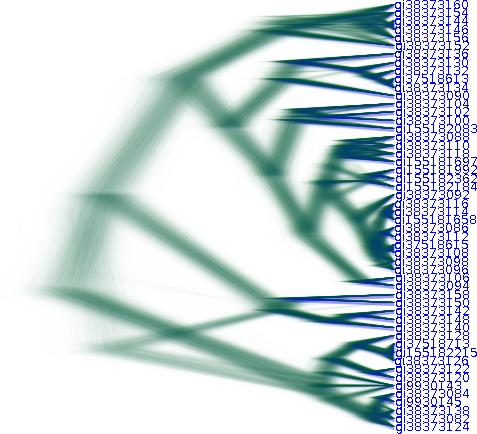
\includegraphics[width=0.3\textwidth]{DensiTreeExample2.jpg}
    };
    \node[state] (HL) [above left=-0.25cm and -0.25cm of H, fill=white] {
      6
    };   
    \node[state] (I) [rectangle, right of=H] {
      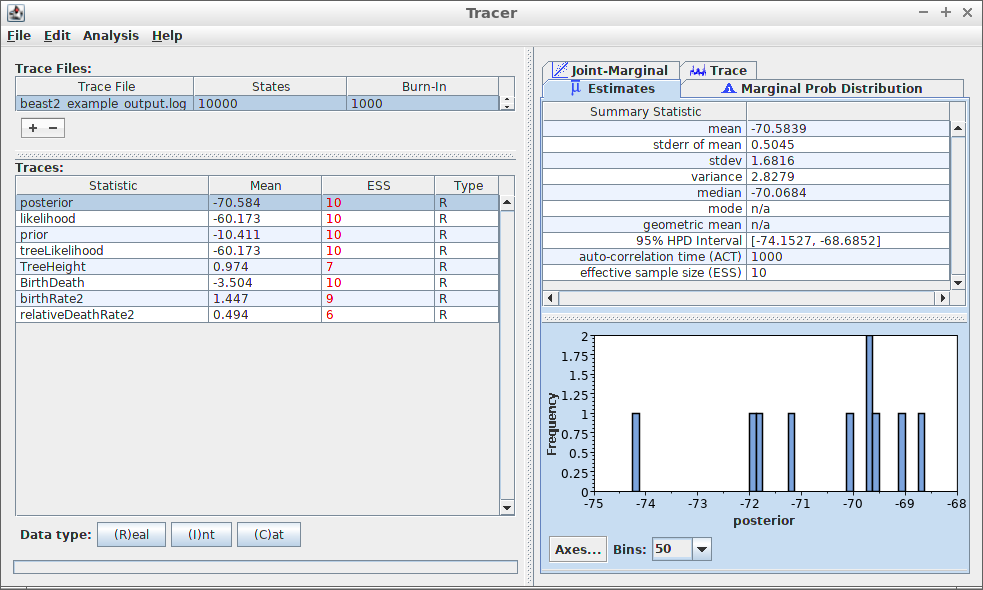
\includegraphics[width=0.6\textwidth]{tracer_example_output.png}
    };
    \node[state] (IL) [above left=-0.25cm and -0.25cm of I, fill=white] {
      7
    };   
    \path 
      (A) edge [anchor = west] node {} (E)
      (E) edge [anchor = west] node {} (F)
      (F) edge [anchor = west] node {} (H)
      (F) edge [anchor = west] node {} (I)
    ; 
    \path [-o,draw] (B) -- ($ (A) !.5! (E) $);
    \path [-o,draw] (C) -- ($ (E) !.5! (F) $);
    \end{tikzpicture}
  }
  \caption{
    Workflow using GUI tools. From an alignment (1) and BEAUti (2), 
    a BEAST2 configuration file (3) is created. BEAST2 (4) uses that file
    to infer a posterior, storing it in multiple files (5). These results
    are visualized using DensiTree (6) and Tracer (7). babette allows
    for the same workflow, all from an R function call.
  }
  \label{fig:workflow}
\end{figure}
%%%%%%%%%%%%%%%%%%%%%%%%%%%%%%%%%%%%%%%%%%%%%%%%%%%%%%%%%%%%%%%%%%%%%%%%%%%%%%%%

%%%%%%%%%%%%%%%%%%%%%%%%%%%%%%%%%%%%%%%%%%%%%%%%%%%%%%%%%%%%%%%%%%%%%%%%%%%%%%%%%%%%%%
\section{Description}
%%%%%%%%%%%%%%%%%%%%%%%%%%%%%%%%%%%%%%%%%%%%%%%%%%%%%%%%%%%%%%%%%%%%%%%%%%%%%%%%%%%%%%

\verb;babette; is written in the R programming language \cite{R}
and enables the full BEAST2 workflow from an R function call,
in a similar way that BEAUti, DensiTree and Tracer do.

\verb;babette;'s main function is \verb;run_beast2;, which, 
configures BEAST2, runs it and parses its output. 
\verb;run_beast2; needs at least the name of a 
FASTA file containing a DNA alignment. 
The default settings for the other arguments of \verb;run_beast2; 
are identical to BEAUti's and BEAST2's default settings.
Per alignment, a site model, clock model and tree prior can be chosen.
Multiple alignments can be used, each with its own (unlinked) site model, 
clock model and tree prior.

\verb;babette; currently has 61 exported functions to set up  
a BEAST2 configuration file. 
\verb;babette; is an alternative for a majority of BEAUti use cases, 
but does not yet support the full functionality of BEAUti. 
Because of BEAUti's high number of plugins, 
\verb;babette; uses a software architecture that expects te be extended.

\verb;babette; has 7 exported function to run and help run BEAST2.
One function is a wrapper function to run BEAST2, others
allow the user to check if a BEAST2 configuration file is indeed valid.

\verb;babette; has 20 exported function to parse the BEAST2 output
files and analyse the created posterior. \verb;babette; gives the
same ESSes and summary statistics as Tracer. The data is formatted
as such, that it can easily be visualized using \verb;ggplot2; (for a trace,
similar to Tracer)
or \verb;phangorn; \cite{phangorn} (for the phylogenies in a posterior, similar to DensiTree). 

%%%%%%%%%%%%%%%%%%%%%%%%%%%%%%%%%%%%%%%%%%%%%%%%%%%%%%%%%%%%%%%%%%%%%%%%%%%%%%%%%%%%%%
\section{Examples}
%%%%%%%%%%%%%%%%%%%%%%%%%%%%%%%%%%%%%%%%%%%%%%%%%%%%%%%%%%%%%%%%%%%%%%%%%%%%%%%%%%%%%%

In R, the functions of a package need to be loaded in the global namespace first:

\begin{lstlisting}[language=R, floatplacement=H]
library(babette)
\end{lstlisting}

BEAUti, and likewise \verb;babette;, needs at least a FASTA filename
to produce a BEAST2 configuration file. 
In BEAUti, this is achieved by loading a FASTA file, 
then saving an output file using a common
save file dialog. After this, BEAST2 needs to be invoked
on the created configuration file to create multiple files
storing the created posterior. Finally, these output
files must be parsed by either Tracer of DensiTree.

In \verb;babette;, the same is achieved by:

\begin{lstlisting}[language=R, floatplacement=H]
out <- run_beast2("alignment.fas")
\end{lstlisting}

This code will create a (temporary) BEAST2 configuration file,
using a FASTA file with name \verb;alignment.fas;, 
using the same default settings as BEAUti.
\verb;babette; will then execute a BEAST2 with that file, and
parses the output. The output, named \verb;out;, is a list of
parameter estimates, posterior phylogenies (one per alignment)
and operator acceptances. 

The default settings for BEAUti (and thus \verb;babette;) are, 
among others, to use a Jukes-Cantor site model \cite{cantor1969mammalian}, 
a strict clock, and a Yule birth tree prior \cite{yule}. 

An example of using a different site model, clock model 
and tree prior is:

\begin{lstlisting}[language=R, floatplacement=H]
out <- run_beast2(
  "alignment.fas",
  site_models = create_hky_site_model(),
  clock_models = create_rln_clock_model(),
  tree_priors = create_bd_tree_prior()
)
\end{lstlisting}

This code uses an HKY site model, a relaxed log-normal clock model and a 
birth-death tree prior, each with their default settings in BEAUti.
Table \ref{tab:functions} shows an overview of all functions to 
create site models, clock models and tree priors.

\begin{table}[]
\centering
\begin{tabular}{ | l | l | }
\hline
\textbf{Name} & \textbf{Description} \\
\hline
\verb;create_beast2_input_file; & Creates a BEAST2 input file \\
\hline
\verb;create_gtr_site_model; & Create a GTR site model \\
\verb;create_hky_site_model; & Create an HKY site model \\
\verb;create_jc69_site_model; & Create a Jukes-Cantor site model \\
\verb;create_tn93_site_model; & Create a TN93 site model \\
\hline
\verb;create_rln_clock_model; & Create a relaxed log-normal clock model \\
\verb;create_strict_clock_model; & Create a strict clock model \\
\hline
\verb;create_bd_tree_prior; & Create a birth-death tree prior \\
\verb;create_cbs_tree_prior; & Create a coalescent Bayesian skyline tree prior \\
\verb;create_ccp_tree_prior; & Create a coalescent constant-population tree prior \\
\verb;create_cep_tree_prior; & Create a coalescent exponential-population tree prior \\
\verb;create_yule_tree_prior; & Create a Yule tree prior \\
\hline
\verb;create_beta_distr; & Create a beta distribution \\
\verb;create_exp_distr; & Create an exponential distribution \\
\verb;create_gamma_distr; & Create a gamma distribution \\
\verb;create_inv_gamma_distr; & Create an inverse gamma distribution \\
\verb;create_laplace_distr; & Create a Laplace distribution \\
\verb;create_log_normal_distr; & Create a log-normal distribution \\
\verb;create_normal_distr; & Create a normal distribution \\
\verb;create_one_div_x_distr; & Create a 1/X distribution \\
\verb;create_poisson_distr; & Create a Poisson distribution \\
\verb;create_uniform_distr; & Create a uniform distribution \\
\hline
\end{tabular}
\caption{babette's main functions}
\label{tab:functions}
\end{table}

Note that the arguments' names \verb;site_models;, \verb;clock_models; 
and \verb;tree_priors; are plural, as each of these
can be (a list of) one or more elements. Each of these arguments must 
have the same number of elements, so that each alignment has its
own site model, clock model and tree prior. 

An example of two alignments, each with its own site model, is:

\begin{lstlisting}[language=R, floatplacement=H]
out <- run_beast2(
  c("anthus_aco.fas", "anthus_nd2.fas"),
  site_models = list(
    create_tn93_site_model(), 
    create_gtr_site_model()
  )
)
\end{lstlisting}

\verb;babette; also uses the same default distributions as BEAUti 
for the site models, clock models and tree priors. 
For example, a Yule tree prior assumes the birth rate follows a uniform distribution, 
from minus infinity to plus infinity. 
This assumption implies that negative and positive birth rates are just as likely, 
where a negative birth rate is biologically impossible (note that 
in practice, this usually works out just fine).
One may prefer an exponential distribution instead, 
as this would assume only positive birth rates, 
and makes high birth rates unlikely.

The following script shows how to do this in \verb;babette;:

\begin{lstlisting}[language=R, floatplacement=H]
out <- run_beast2(
  "alignment.fas",
  tree_priors = create_yule_tree_prior(
    birth_rate_distr = create_exp_distr()    
  )
)
\end{lstlisting}

Our initial motivation to create \verb;babette; 
is that we wanted to fix the crown age of a phylogeny.
BEAUti assumes that a phylogeny has a crown age that needs to be jointly-estimated
with the phylogeny and other parameters. It does not allow for fixing
the crown age. Without \verb;babette;, one needs to manually edit the BEAST2 
configuration file, which is tedious and prone to errors. 
Fixing the crown ages is especially useful for theoretical experiments,
as this allows for one less source of variation.

This is how to specify a fixed crown age with \verb;babette;:

\begin{lstlisting}[language=R, floatplacement=H]
out <- run_beast2(
  "alignment.fas",
  posterior_crown_age = 15
)
\end{lstlisting}

\verb;babette; allows for the same functionality of Tracer. 
Tracer, among others, shows the effective sample
sizes of each posterior's variables. As an MCMC run needs to
converge first, Tracer discards the first 10\% of all parameter
estimates. This is called the burn-in. To calculate the effective
sample sizes in \verb;babette;, with the same burn-in of 10\%:

\begin{lstlisting}[language=R, floatplacement=H]
traces <- remove_burn_ins(traces = out$estimates, burn_in_fraction = 0.1)
esses <- calc_esses(traces, sample_interval = 1000)
\end{lstlisting}

Tracer displays multiple summary statistics for each
estimated variable: the mean and its standard error, standard deviation,
variance, median, mode, geometric mean, 95\% highest posterior density interval, 
auto-correlation time and effective sample size. To obtain all these summary statistics 
of, for example, the estimated birth rate in \verb;babette;:

\begin{lstlisting}[language=R, floatplacement=H]
sum_stats <- calc_sum_stats(
  out$estimates$birthRate, 
  sample_interval = 1000, 
  burn_in_fraction = 0.1
)
\end{lstlisting}

\verb;babette; allows for the same functionality of DensiTree.
DensiTree displays the phylogenies in a posterior at the same
time scale over one another, allowing to see the uncertainty in
topology and branch lengths. To visualize the same in \verb;babette;:

\begin{lstlisting}[language=R, floatplacement=H]
densitree(out$anthus_aco_trees)
\end{lstlisting}

%%%%%%%%%%%%%%%%%%%%%%%%%%%%%%%%%%%%%%%%%%%%%%%%%%%%%%%%%%%%%%%%%%%%%%%%%%%%%%%%%%%%%%
\section{babette development and other resources}
%%%%%%%%%%%%%%%%%%%%%%%%%%%%%%%%%%%%%%%%%%%%%%%%%%%%%%%%%%%%%%%%%%%%%%%%%%%%%%%%%%%%%%

\verb;babette; is free, libre and open source software available from the official R package archive at 
\url{http://cran.r-project.org/src/contrib/PACKAGES.html\#babette}
and is licensed under the GNU General Public License v3.0.

\verb;babette; uses the Travis CI \cite{travis} 
continuous integration service, which is known to significantly 
increase the the number of bugs exposed \cite{vasilescu2015} and increases
the speed at which new features are added \cite{vasilescu2015}.
\verb;babette; has a 100\% code coverage, which correlates with code quality \cite{horgan1994,del1995correlation}. 
\verb;babette; follows Hadley Wickham's style guide \cite{style_guide}, which improves software quality \cite{fang2001}.
\verb;babette; is dependent on multiple packages, which are 
\verb;APE; \cite{APE}, 
\verb;beautier; \cite{beautier},
\verb;beastier; \cite{beastier},
\verb;devtools; \cite{devtools},
\verb;geiger; \cite{GEIGER},
\verb;ggplot2; \cite{ggplot2},
\verb;knitr; \cite{knitr},
\verb;phangorn; \cite{phangorn},
\verb;rmarkdown; \cite{rmarkdown},
\verb;seqinr; \cite{seqinr},
\verb;stringr; \cite{stringr},
\verb;testit; \cite{testit} and 
\verb;tracerer; \cite{tracerer} and
\verb;TreeSim; \cite{TreeSim}.

\verb;babette;'s development takes place on GitHub \cite{github},
\url{https://github.com/richelbilderbeek/babette}, 
which accommodates collaboration \cite{perez2016ten} 
and improves transparency \cite{gorgolewski2016practical}.
\verb;babette;'s GitHub facilitates feature requests and has guidelines how to do so.

\verb;babette;'s documentation is extensive. All functions are documented
in the package's internal documentation. For quick use, 
each exported function shows a minimal example. 
For easy exploration, each exported function's documentation links to related functions.
Additionally, \verb;babette; has a vignette that demonstrates extensively how
to use it. The GitHub documentation helps to get started, with a dozen examples 
of BEAUti screenshots with equivalent \verb;babette; code.

%%%%%%%%%%%%%%%%%%%%%%%%%%%%%%%%%%%%%%%%%%%%%%%%%%%%%%%%%%%%%%%%%%%%%%%%%%%%%%%%%%%%%%
\section{Citation of babette}
%%%%%%%%%%%%%%%%%%%%%%%%%%%%%%%%%%%%%%%%%%%%%%%%%%%%%%%%%%%%%%%%%%%%%%%%%%%%%%%%%%%%%%

Scientists using \verb;babette; in a published paper can cite this
article, and/or cite the \verb;babette; package 
directly. To obtain this citation from within an R script, use:

\begin{lstlisting}[language=R]
> citation("babette")
\end{lstlisting}

%%%%%%%%%%%%%%%%%%%%%%%%%%%%%%%%%%%%%%%%%%%%%%%%%%%%%%%%%%%%%%%%%%%%%%%%%%%%%%%%%%%%%%
\bibliographystyle{plain}
\bibliography{article}
%%%%%%%%%%%%%%%%%%%%%%%%%%%%%%%%%%%%%%%%%%%%%%%%%%%%%%%%%%%%%%%%%%%%%%%%%%%%%%%%%%%%%%

\end{document}
\grid
